\documentclass{article}
\usepackage[osf,tabular,sfdefault]{biolinum}
\usepackage[scale=.75]{FiraMono}
\usepackage[onehalfspacing]{setspace}
\usepackage{sfmath,amsmath,bm}
\usepackage[marginal]{footmisc}
% shorthands
\usepackage[
  colorlinks,
  linkcolor=blue,
  citecolor=magenta,
]{hyperref}
\usepackage{xspace}
\newcommand{\covid}{\mbox{\textsc{covid-19}}\xspace}
\newcommand{\polymod}{\mbox{\textsc{polymod}}\xspace}
\newcommand{\hreftt}[1]{\href{#1}{\texttt{#1}}}
\setlength{\skip\footins}{\bigskipamount}
\newcommand{\rom}[1]{\textsc{\romannumeral#1})}
% bib
\addbibresource{refs}
% floats
\usepackage{graphicx}
\graphicspath{{fig/}}
\usepackage{booktabs}
\usepackage{subcaption}
\newcommand{\floatfoot}[2][1]{%
  \par\parbox{#1\linewidth}{\footnotesize#2}}

\begin{document}
  \maketitle
  \section{Objective}\label{s:obj}
  Consider a population stratified by into
  $A=11$ age groups ($a$) and $N=510$ neighbourhoods (FSA, $n$).
%  A proportion $\e_n$ of individuals in FSA $n$ are essential workers.
  We are interested in defining the number of contacts formed between
  all individuals in group $an$ and all individuals in group $a'n'$,
  which we denote $X_{ana'n'}$.
  Then, we will use a pre-determined assignment FSAs into $G=10$ groups ($g$)
  to aggregate the FSA dimensions and obtain $X_{aga'g'}$.
  \section{Approach}\label{s:methods}
  \subsection{Data}\label{ss:data}
  The \textsc{polymod} study estimates the average numbers of contacts per person per day
  between age groups $a$ and $a'$, stratified by the following types ($y$) of contacts:
  \emph{home}, \emph{work}, \emph{school}, \emph{transport}, \emph{leisure}, \emph{other};
  these data are denoted $C_{aa'y}$ and are illustrated in Figure~\ref{fig:polymod}
  We assume these rates of contacts are similar for our population
  (see Section~\ref{ss:caveats} for further comment on these assumptions).
%  , with the following adjustment.
%  We assume that essential workers have more \emph{work} and \emph{home} contacts
%  than non-essential workers, by a factor of $f_{y\e}$,
%  due to the work environment and multi-generational households, respectively.
%  Later, we will also consider differences in the ability to reduce daily contacts
%  following lockdown orders, etc.
%  \par
  The total number of type $y$ contacts formed by people in age group $a$ is
  $C_{ay} = \sum_{a'} C_{aa'y}$.
  We know the sizes of populations in each FSA $n$, stratified by age groups $a$,
  which we denote $P_{na}$.
  Thus, the total number of type $y$ contacts made available by FSA $n$ is:
  \begin{equation}
    Q_{ny} = P_{na} \times C_{ay}
    \label{eq:Q.ny}
  \end{equation}
  \par
  Cell phone (\textsc{tbc}) mobility data from Ontario has been used to estimate
  the average proportion of individuals residing in FSA $n$ who travel to FSA $n'$ per day,
  denoted $B^*_{nn'}$.
  These proportions are aggregated into groups $gg'$ and shown in Figure~\ref{fig:mobility}.
  To use these data, we need to make several assumptions:
  1)~What proportion of the FSA population are captured in the data?
  2)~Is this proportion equally distributed across age groups and equal across FSAs?
  3)~With whom do travellers mix in the destination FSA: local residents and/or other travellers?
  4)~What types of contacts are formed where?
  \par
  For now, we assume that:
  (1,2) the mobility data sample an equal proportion $b_s$ across all FSA and age groups; and
  (3,4) a proportion of type $y$ contacts $b_y$ are formed
  either while travelling or with travellers to FSA $n$,
  and the remainder $(1-b_y)$ are formed only with other locals in FSA $n$.
  The proportion of people travelling between FSAs $n$ and $n'$
  after correcting for under-sampling of mobility data is therefore $B_{nn'} = B^*_{nn'}/b_s \le 1$,
  and the total proportion of people travelling away from FSA $n$ per day is $B_n = \sum_n B_{nn'}$.
  \subsection{Numbers of Contacts}\label{ss:math}
  Consider $Q_{ny}$: the total number of type $y$ contacts formed by individuals in FSA $n$.
  These contacts can be formed with three pools of potential ``others'':
  (a) others met while travelling to other FSAs;
  (b) others met who travelled to this FSA; and
  (c) others from this FSA (who may/not also travel at other times to form other types of contacts).
  The total contacts $Q_{ny}$ are distributed between (a,b,c) as follows:
  \begin{equation} 
    Q_{ny} \sim \begin{cases}
      B_n b_y     & \textrm{(a) while travelling} \\
      (1-B_n) b_y & \textrm{(b) with local traveller pool} \\
      (1-b_y)     & \textrm{(c) with locals only} \\
    \end{cases}
  \end{equation}
  Now consider the local traveller pool in FSA~$n^*$ (a,b).
  The total number of type $y$ contacts made available to this pool by FSA $n$ is
  (where $1_{x=y}$ denotes $1$ if $x=y$ else $0$):
  \begin{equation}
    Q^{n^*}_{ny} = b_y Q_{ny} \big( B_{nn^*} + 1_{n=n^*} (1-B_n) \big)
  \end{equation}
  So, the total number of contacts made available to the pool from all FSAs is:
  \begin{equation}
    T_{n^*y} = \sum_{n} Q^{n^*}_{ny}
  \end{equation}
  If random mixing is assumed within the traveller pool,
  then the total number of contacts formed between
  individuals from FSAs $n$ and $n'$ in the pool is:
  \begin{equation}
    X^{n^*}_{nn'y} = \frac{Q^{n^*}_{ny} \thinspace Q^{n^*}_{n'y}}{T_{n^*y}}
  \end{equation}
  The total number of contacts formed between FSA $n$ and FSA $n'$ is therefore
  the sum across all traveller pools, including those corresponding to $n=n^*$ and $n'=n^*$,
  plus the local contacts from case (c):
  \begin{equation}
  X_{nn'y} = \sum_{n^*} X^{n^*}_{nn'y} + 1_{n=n'}\big( (1-b_y) Q_{ny} \big)
  \end{equation}
  \subsection{Free Parameters}\label{ss:params}
  The free parameters (count) introduced here are:
  \begin{itemize}
    \item $b_s$: (1) the proportion of individuals represented in the mobility data
    \item $b_y$: (6) the proportion of type $y$ contacts that are formed with the traveller pool
  \end{itemize}
  However, some values of $b_y$ can likely be fixed, such as
  $b_1 = 0$: no \emph{home} contacts formed with the traveller pool;
  $b_2 = 1$: all \emph{work} contacts formed with the traveller pool, etc.
  \pagebreak
  \subsection{Caveats}\label{ss:caveats}
  \begin{itemize}
    \item We assume that travelling individuals only form contacts in one destination.
          However, due to the large numbers involved,
          this assumption won't likely have any influence on the results.
    \item We have not considered differences in contact numbers by FSA $n$,
          for example, due to different types of employment or housing.
          However, this could be added to $Q_{ny}$ in Eq.~(\ref{eq:Q.ny}).
    \item The proportion of contacts that are formed internally (within the same FSA)
          is sensitive to the parameter $b_s$ because
          a large non-mobile population in FSA $n^*$ (locals) will dominate the local traveller pool.
    \item Our current approach aggregates over age strata before calculating
          the contacts formed between FSA for simplicity, thus precluding age:FSA interactions in mixing.
          However, since contact types are disaggregated,
          age:contact-type interactions could be supported.
  \end{itemize}
  \section{Results}\label{s:results}
  In Section~\ref{s:methods} we described the methodology in relation to $N=510$ FSAs.
  However, as noted in Section~\ref{s:obj}, we eventually intended to aggregate the mixing matrices
  to reflect $G=10$ groupings of FSAs.
  Since the mobility data currently available are based on these groupings ($g$),
  the results below are for the groupings.
  When analyzing groups $g$ instead of FSAs $n$,
  the methodology above can be repeated exactly using $n \rightarrow g$,
  $Q_{ny} \rightarrow Q_{gy}$, and $B_{nn'} \rightarrow B_{gg'}$,
  which can be obtained as suggested in v.1 of this report
  (where $S_g$ is the set of $n$ assigned to group $g$):
  \begin{equation}
    Q_{gy} = \sum_{n \in S_g} Q_{ny},\quad
    B_{gg'} = \sum_{n \in S_g} \sum_{n' \in S_{g'}} B_{nn'}
  \end{equation}
  \par
  Figure~\ref{fig:Xggy} illustrates the total number of contacts (millions)
  predicted between deciles, stratified by contact type,
  using $b_s = .05$ and $b_y = [0,1,0,1,\frac{1}{2},\frac{1}{2}]$.
  We verified that $\sum_{g'} {X_{gg'y}} = Q_{gy}$ for all contact types $y$.
  When $b_y = 0$ (e.g. \emph{home} contacts), the contact matrix has no off-diagonal elements.
  However, even for $b_y = 1$ (e.g. \emph{work} contacts),
  the contact matrix is still dominated by the diagonal
  due to the tendency for individuals to move between FSA in the same decile
  (Figure~\ref{fig:mobility}),
  and the larger size of the non-mobile population (locals) in the local traveller pool.
  The proportions of all contacts formed within the same decile across the various contact types was:
  \emph{home}: 1.00, \emph{work}: 0.15, \emph{school}: 1.00, \emph{transport}: 0.15, \emph{leisure}: 0.58, \emph{other}: 0.58;
  and 0.64 overall.
  To improve readability, Figure~\ref{fig:Xggy} therefore also shows the number of contacts
  in the off-diagonal elements alone.
  Finally, Figure~\ref{fig:Xgg} similarly illustrates the total number of contacts (millions)
  predicted between deciles, after aggregating over contact types.
  \begin{figure}
    \centering
    \includebiggraphics{Xggy.pdf}
    \includebiggraphics{Xggy-o.pdf}
    \caption{Total number and types of contacts formed between deciles (millions);
      raw values (top) and after removing the dominant diagonal (bottom)}
    \label{fig:Xggy}
  \end{figure}
  \begin{figure}
    \centering
    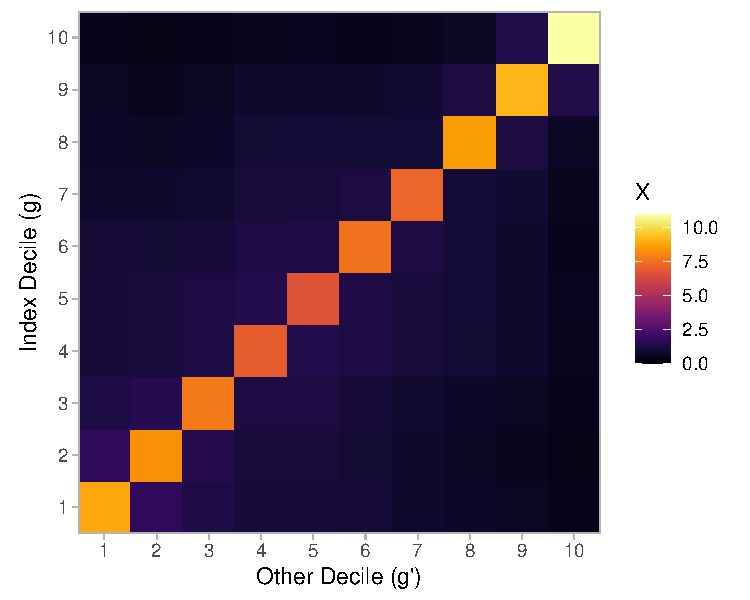
\includegraphics[width=.5\linewidth]{Xgg.pdf}%
    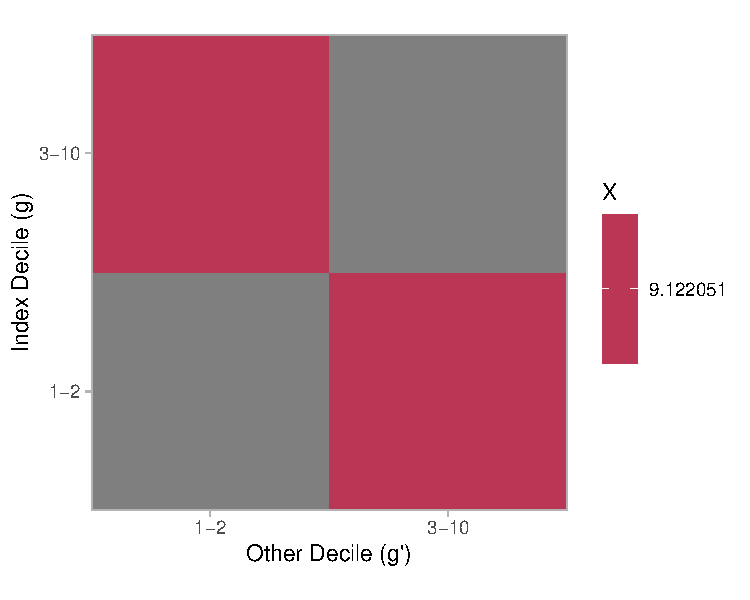
\includegraphics[width=.5\linewidth]{Xgg-o.pdf}
    \caption{Total number of contacts formed between deciles (millions);
      raw values (left) and after removing the dominant diagonal (right)}
    \label{fig:Xgg}
  \end{figure}
  \appendix
  \section{Supplemental Results}
  \begin{figure}[h]
    \centering
    \includebiggraphics{polymod.pdf}
    \caption{Average number and types of contacts between various age groups per day (\textsc{polymod})}
    \label{fig:polymod}
  \end{figure}
  \begin{figure}[h]
    \centering
    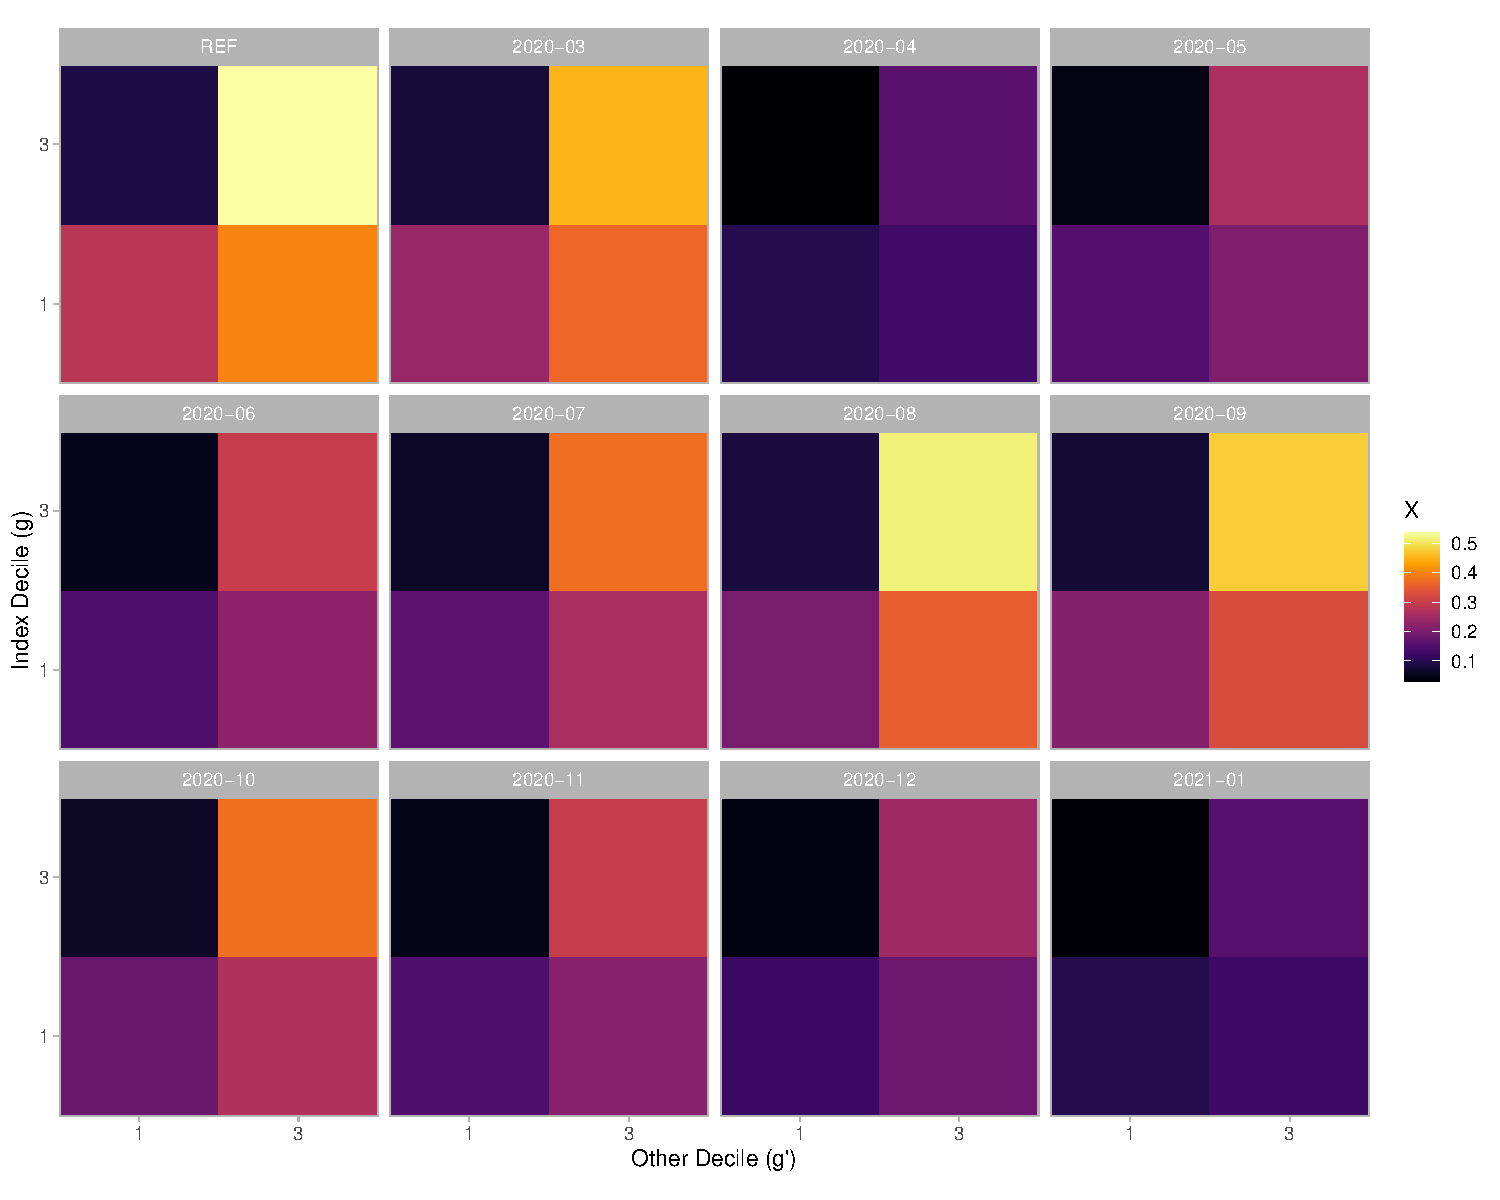
\includegraphics[width=.4\linewidth]{mobility.pdf}
    \caption{Raw cell phone mobility data:
      proportion of individuals residing in ``index decile'' who travelled to ``other decile'' per day}
    \label{fig:mobility}
  \end{figure}
\end{document}